% !TEX root = Bachelorarbeit_Paul_Zilewitsch.tex
\section{Konzipierung}
\subsection{Analyse aus Kapitel 1 und Kapitel 2 (UML-Diagramme etc.)}
\subsection{Zielsetzung}
\subsection{Sicherheitsaspekte}
\noindent
Immer wieder vernachlässigen Entwickler die Sicherheit ihrer Implementierungen. Das liegt meistens an mangelnder Zeit, da Releases einen festen Zeitplan verfolgen, den es einzuhalten gilt. Es kann aber auch sein, dass die Implementierung nicht aus dem Blickwinkel der Sicherheit betrachtet wird. "Hauptsache es funktioniert erst einmal", wird dann häufig als Argument genutzt. Natürlich hat das wenig mit Sicherheit zu tun. Dabei können es Entwickler mit wenig Aufwand, Angreifern deutlich schwerer machen. Deswegen werden im nachfolgendem zwei Sicherheitsprobleme für die Umsetzung des Konzepts in GEBman 10 besprochen. Die Abbildung XX zeigt zwei kritische Bereiche, die genauer erläutert werden müssen.

\begin{figure}[h!]
\centering
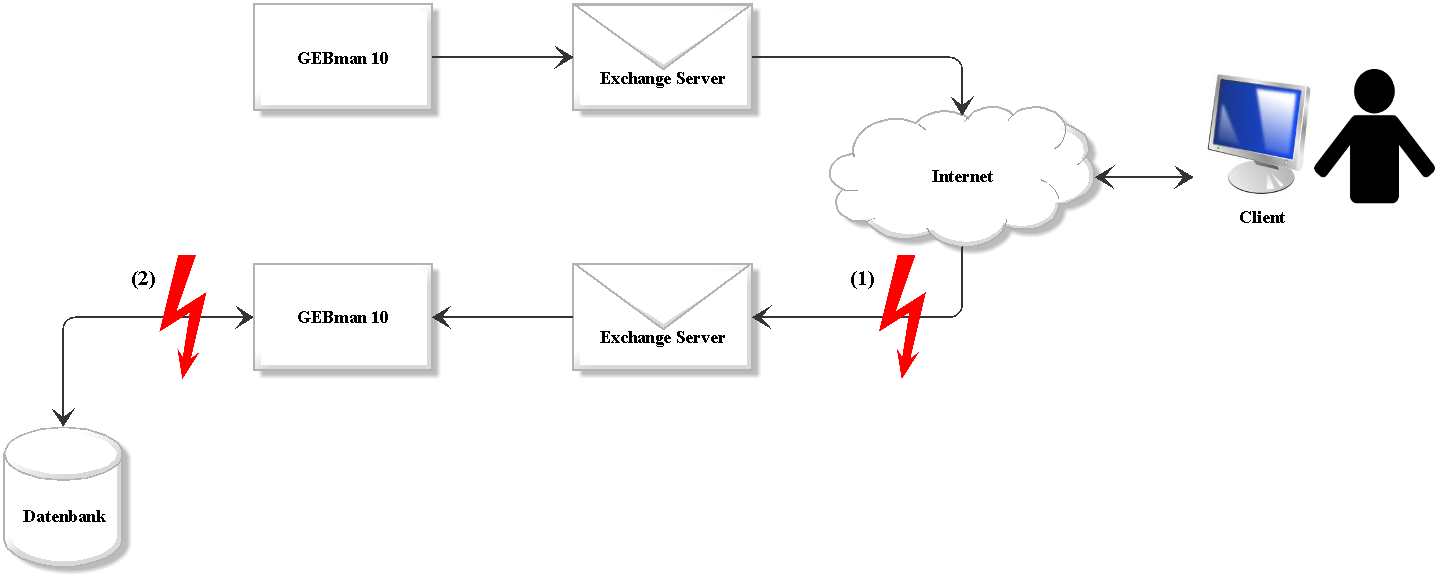
\includegraphics[width=0.85\textwidth]{Abbildungen/Sicherheitsprobleme.png}
	\caption[Sicherheitsprobleme]{Sicherheitsprobleme, Quelle:eigene Darstellung}
	\label{fig:Sicherheitsprobleme}
\end{figure}

\noindent
Der rechte rote Blitz - gekennzeichnet mit der (1) - symbolisiert das erste Problem.

\noindent
Beim zweiten roten Blitz der Abbildung XX - gekennzeichnet mit der (2) - wird uns die Arbeit nicht wie beim ersten kritischen Bereich abgenommen. GEBman 10 synchronisiert in regelmäßigen Abständen die Nachrichten vom hinterlegten Exchange Server. Entsprechend ihrer ID werden die Nachrichten in die Datenbank von GEBman 10 gespeichert. Nun könnte ein Angreifer beispielsweise versuchen, in den Mail-Body versteckte SQL -Anweisungen oder JavaScript-Code einzuschleusen. Werden die SQL-Anweisungen in die Datenbank geschrieben, ohne sie vorher zu validieren, könnte der Angreifer Informationen über Daten in der Datenbank erlangen. Im schlimmsten Fall könnte er sie zerstören. Diese Angriffstmethode nennt sich SQL-Injection und zielt darauf ab, die normalen SQL-Statements mittels Sonderzeichen zu manipulieren. Selbst einfache Zeichen wie "--" können bewirken, dass alles, was hinter den beiden Bindestrichen steht, ignoriert wird. In T-SQL sind die beiden Bindestriche das Zeichen für einen Kommentar.
\noindent
Bei JavaScript-Code haben wir ein ähnliches Problem mit bestimmten Zeichen. Wird zum Beispiel die einfache Zeichenfolge "<script>alert('hallo')<script>" in die Datenbank geschrieben, passiert ersst einmal gar nichts. Die SQL-Statements werden hierdruch nicht manipuliert. Doch wird diese Zeichenfolge beispielsweise als Antwort auf eine Meldung geladen, erkennt der Browser möglicherweise JavaScript-Code anstatt einfachen Text. Das hat in unserem Beispiel zur Folge, dass der Browser eine kleine Nachricht meldet (siehe Abbildung).
Auch hier muss vor dem Einfügen der Zeichenfolge, eine Validierung vollzogen werden. Welche Zeichen genau gefiltert werden müssen, wird im Punkt 5 Umsetzung erläutert. Man sollte sich jedoch nicht darauf verlassen, dass die Schutzmechanismen des Microsoft Exchange Servers alle Zeichen und Zeichenfolgen als Bedrohung erkennen. Zeichen wie "--" oder ">" können durchaus im normalen Schriftverkehr gebräuchlich sein.
\noindent
Es gibt für Angreifer noch mehr Angriffsmöglichkeiten beispielsweise zwischen Client und Internet/Server über Man-in-the-Middle etc.. Darauf soll aber in dieser Arbeit nicht weiter eingegangen werden, da das ein sehr umfangreiches Thema ist und eine eigenständige Bachelorarbeit bilden könnte. Eins sollte jedem klar sein: Hat ein Cracker genügend Zeit und Ressourcen, ist ein System, das über das Internet kommuniziert, äußert schwer vollkommen zu sichern. 
\noindent
Durch die Analyse aus Punkt 2 und Punkt 3 konnte ein genaues Ziel gesetzt werden. Die Funktionsweise der Exchange Web Services sind geklärt und auch Sicherheitsaspekte wurden berücksichtigt. Die Konzipierung ist somit abgeschlossen und er Implementierung steht nichts mehr im Wege.
